\documentclass[10pt, aspectratio=168]{beamer}
\usepackage[utf8]{inputenc}
\usepackage{xeCJK}
\usepackage{graphicx}
\usepackage {mathtools}
\usepackage{utopia} %font utopia imported
\usetheme{CambridgeUS}
\usecolortheme{dolphin}

% set colors
\definecolor{Verdigris}{RGB}{104,176,171}
\definecolor{Sage}{RGB}{143,192,169}
\definecolor{TeaGreen}{RGB}{200,213,185}
\definecolor{PayneGrey}{RGB} {105,109,125}
\definecolor{Eggshell}{RGB}{250,243,221}
\setbeamercolor*{palette primary}{bg=TeaGreen, fg= PayneGrey}
\setbeamercolor*{palette secondary}{bg=Sage, fg = white}
\setbeamercolor*{palette tertiary}{bg=Verdigris, fg = white}
\setbeamercolor*{titlelike}{fg=Verdigris}
\setbeamercolor*{title}{bg=Verdigris, fg = white}
\setbeamercolor*{item}{ fg=Verdigris}
\setbeamercolor*{caption name}{fg=Verdigris}
\usefonttheme{serif}
\usepackage{natbib}
\usepackage{hyperref}
%------------------------------------------------------------
%titlepage
\setbeamerfont{title}{size=\Large}
\setbeamerfont{subtitle}{size=\small}
\setbeamerfont{date}{size=\small}
\setbeamerfont{institute}{size=\small}
\title [EMP Analysis]{Modeling Electromagnetic Pulse Interactions with Earth's Ionosphere and Magnetic Field}
\author{Atlas Hussey}
\institute[]{ Institute for Computing in Research \\ Santa Fe, NM}
\date[07/29/2025]
{July 29, 2025}

%------------------------------------------------------------

\begin{document}
%The next statement creates the title page.
\frame{\titlepage}

%------------------------------------------------------------
\section{How are EMPs Born?}

    \begin{frame}{How are radio waves propagated?}
    \begin{columns}
        \begin{column}{0.4\textwidth}
            \begin{itemize}
                \item \large{In order to propagate radio waves, you must generate a strong electric current. }
                \vspace{1cm}
                \item Several sources: Nuclear blasts, lightning strikes.
            \end{itemize}  
        \end{column}
        \begin{column}{0.4\textwidth}
             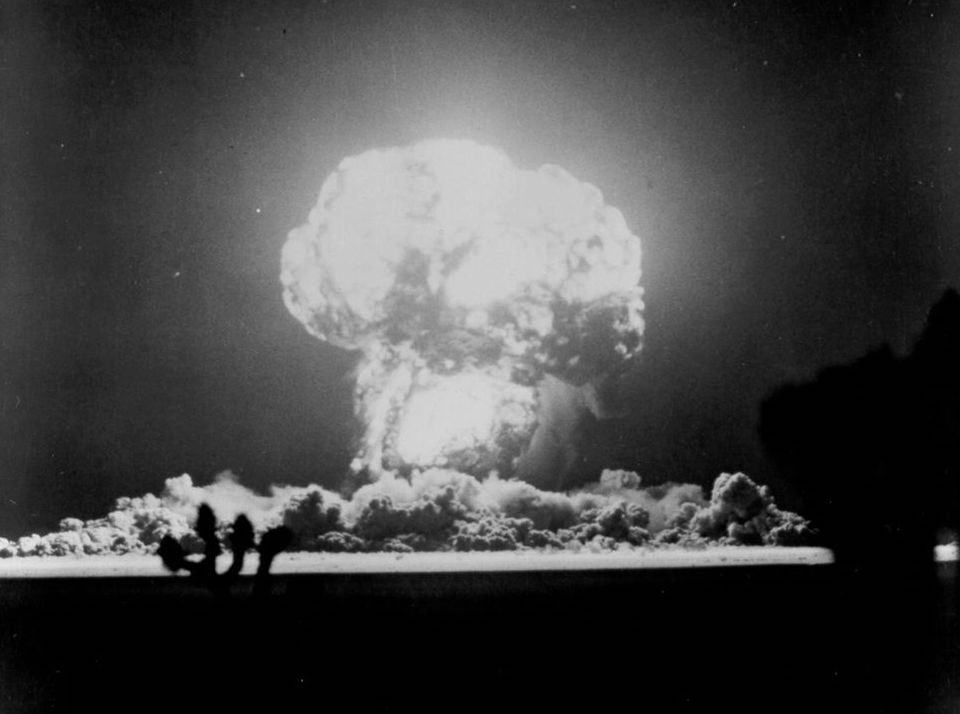
\includegraphics[width=5cm]{apple-2-nuke-test.jpg}
            \caption{\scriptsize{\textit{Source: NPR}}}
            \vspace{0.5cm}
             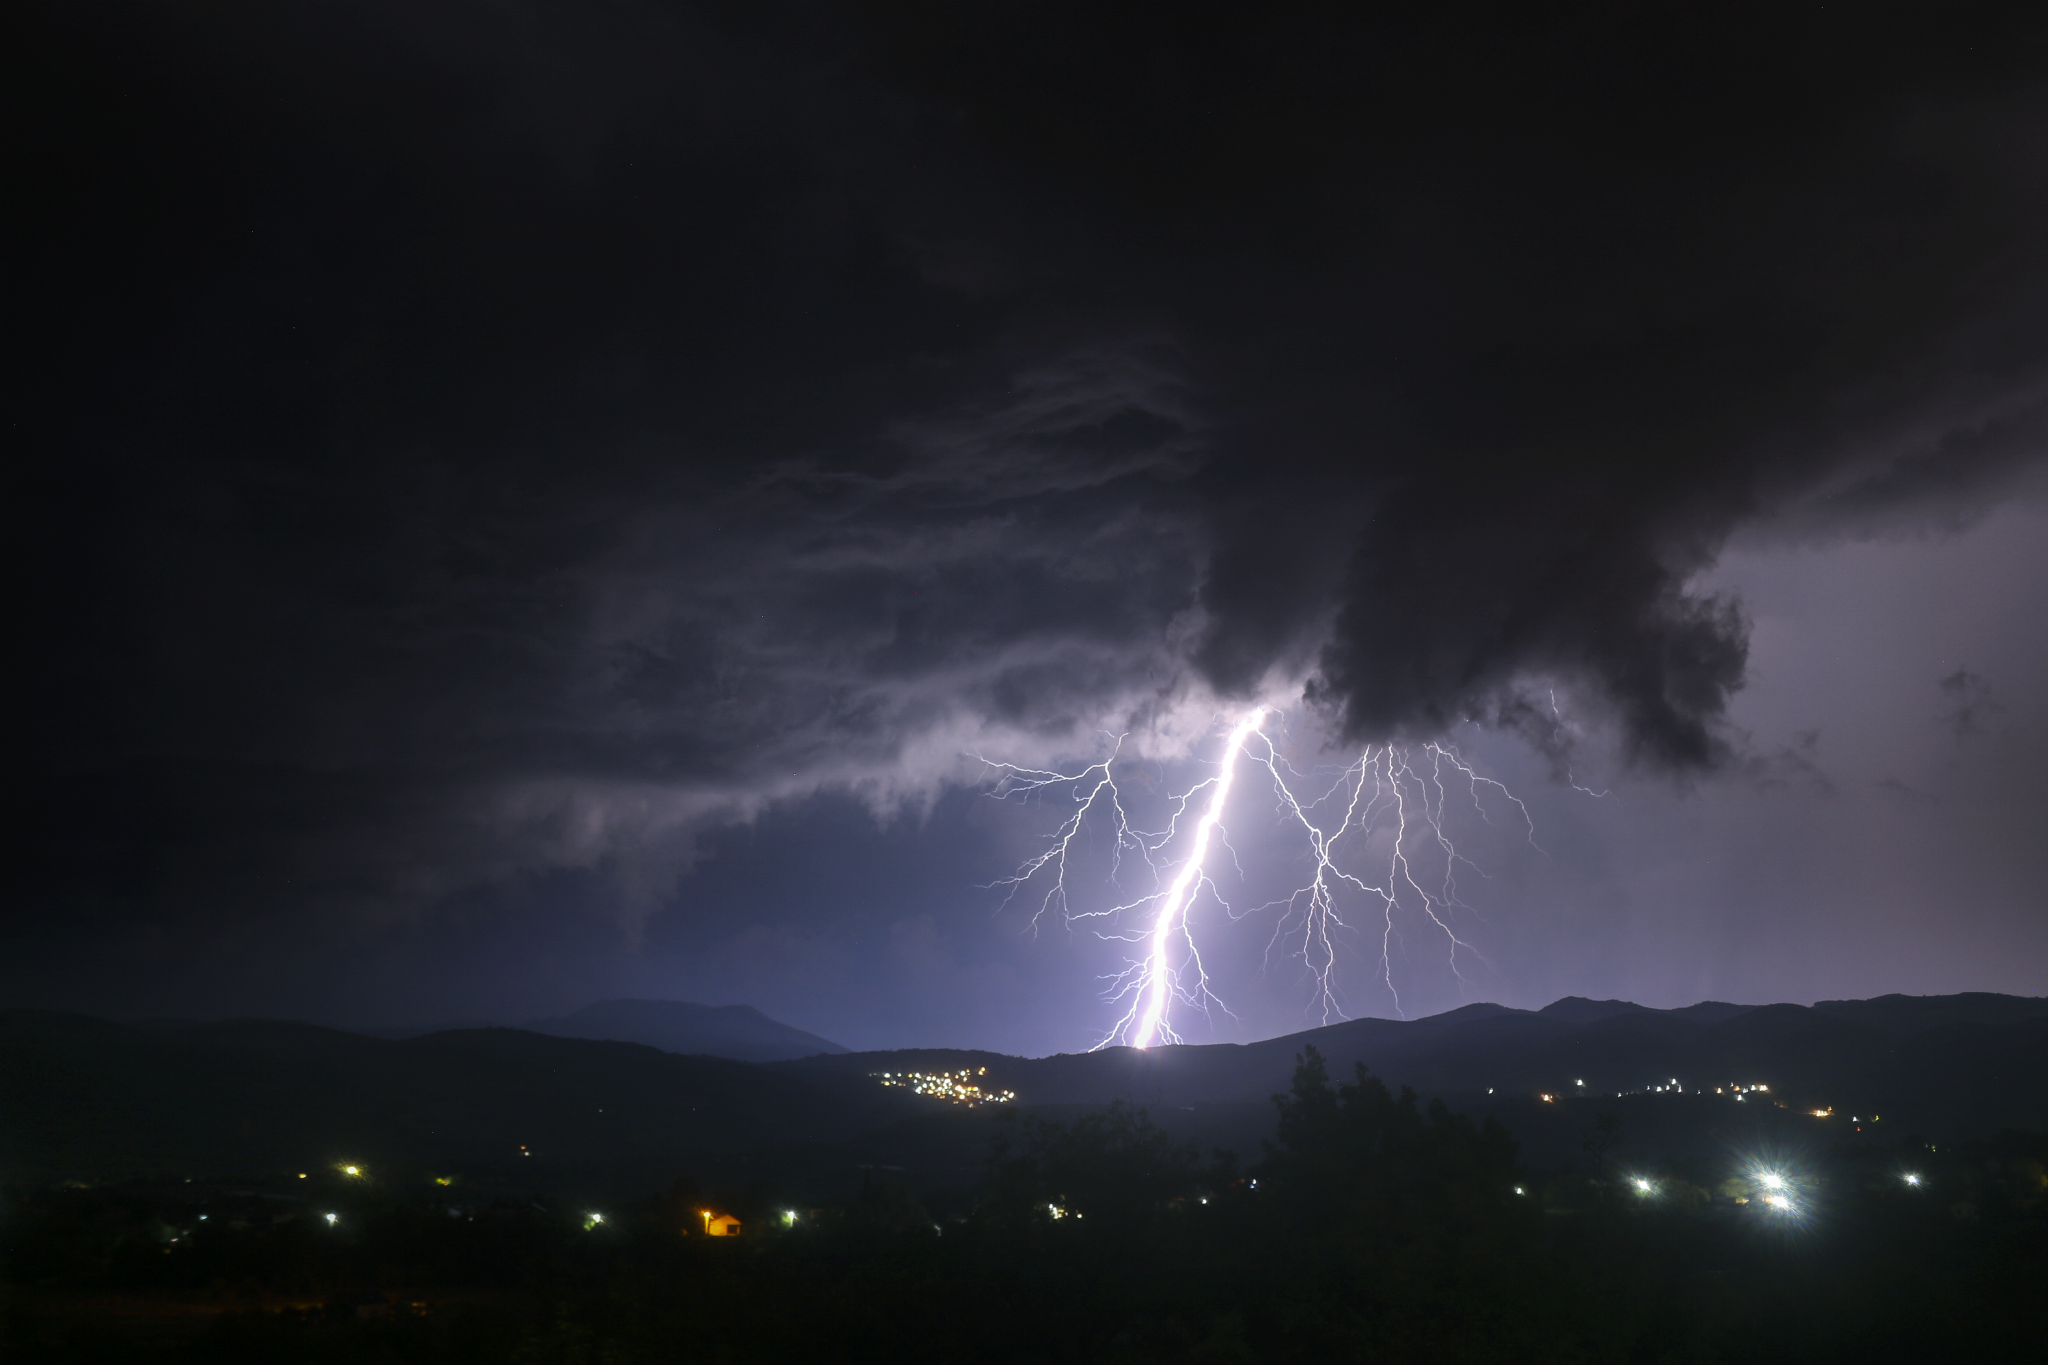
\includegraphics[width=5cm]{Rural_nightime_lightning_strike.png}
            \caption{\scriptsize{\textit{Source: Wikipedia}}}
        \end{column}
    \end{columns}
    \end{frame}
    
    \begin{frame}{Modelling the initial signal}
    \begin{columns}
        \begin{column}{0.4\textwidth}    
            \begin{figure}[h]
                \centering
                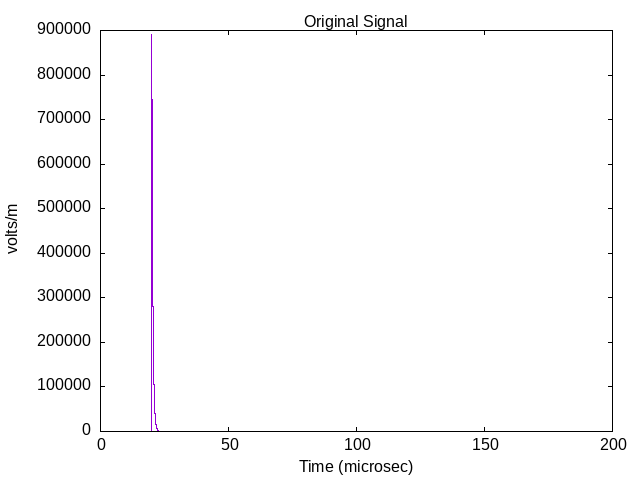
\includegraphics[width=1\textwidth]{emp_original_signal.png}
                \caption{The initial EMP signal without interference from Earth's Ionosphere.}
                \label{fig:emp_original_signal}
            \end{figure}
        \end{column}
        \begin{column}{0.4\textwidth}   
            \begin{itemize}
                \item \large An EMP source usually has a fast rise in frequency, and a slower fall.
                \vspace{0.5cm}
                \item Both rise and fall are exponential functions, so the signal is a "double exponential"
            \end{itemize}
        \end{column}
 \end{columns}
 \end{frame}
    
    \begin{frame}{Interactions with Earth's Ionosphere}
    \begin{itemize}
        \item \large As an EMP passes through the ionosphere, it encounters a varying amount of free electrons
        \item Electrons tend to absorb the energy of frequencies, delaying the speed at which they arrive at the satellite.
        \item Level of delay depends on the wavelength of the frequency.
        \item Extent of delay depends on the total electron content of the atmosphere.
    \end{itemize}
    \end{frame}
    
    \begin{frame}{Interactions with Earth's Magnetic Field}
    \begin{itemize}
        \item \Large The EMP appears to be linear. However, it is actually a sum of two polarizations,
        right-circular and left-circular
        \item Earth's magnetic field separates the two "modes" that travel through the ionosphere at different speeds.
    \end{itemize}
    \end{frame}
    

\section{Modeling a signal}

    \begin{frame}{Fourier Transforms are Useful}
    \begin{itemize}
        \item In order to properly simulate and analyze the changes Earth's ionosphere and magnetic field make to the signal, we must break the signal down into its frequencies.
This can be done using a Fourier Transform.
        \begin{figure}[h]
            \centering
            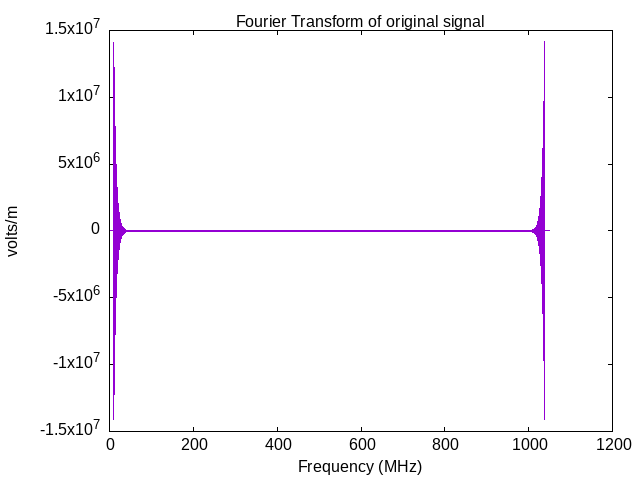
\includegraphics[width=0.4\textwidth]{fft_original_signal.png}
            \caption{Fourier Transform of the initial signal.}
            \label{fig:ft-original-signal}
        \end{figure}
    \end{itemize}
    \end{frame}
    
    \begin{frame}{Fourier Transforms are Useful}
    \begin{columns}
        \begin{column}{0.4\textwidth}    
            \begin{figure}[h]
                \centering
                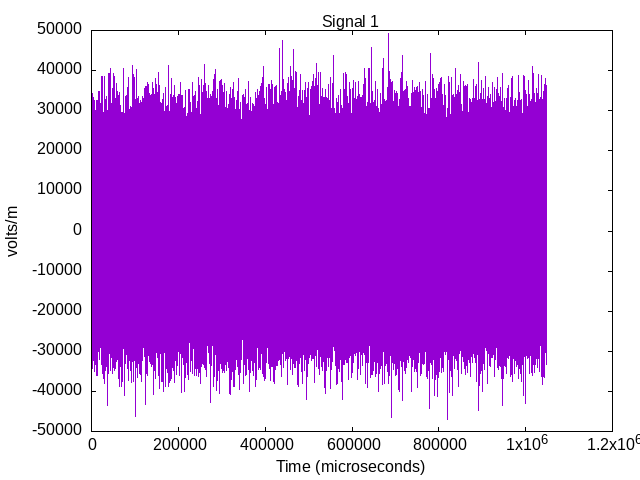
\includegraphics[width=1\textwidth]{test_08.png}
                \caption{Test data}
                \label{fig:test-08}
            \end{figure}
        \end{column}
        \begin{column}{0.4\textwidth}    
            \begin{figure}[h]
                \centering
                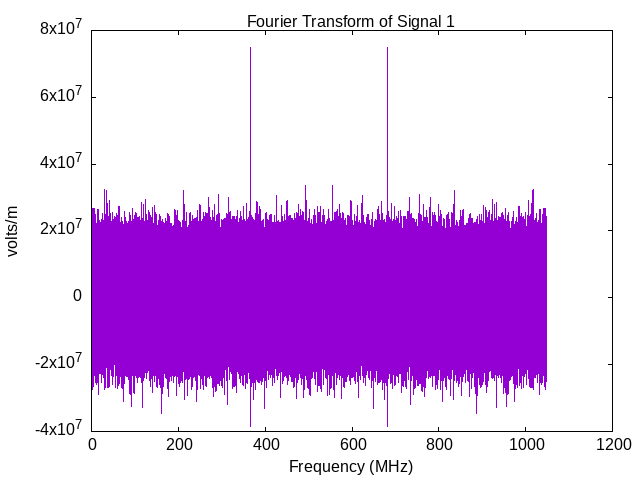
\includegraphics[width=1\textwidth]{fft_test_08.png}
                \caption{Fourier transform of the test data that reveals hidden frequencies}
                \label{fig:fft-test-08}
            \end{figure}
        \end{column}
    \end{columns} 
    \end{frame}
    
    \begin{frame}{Aliasing}
    \begin{columns}
        \begin{column}{0.4\textwidth}
            \begin{figure}[h]
                \centering
                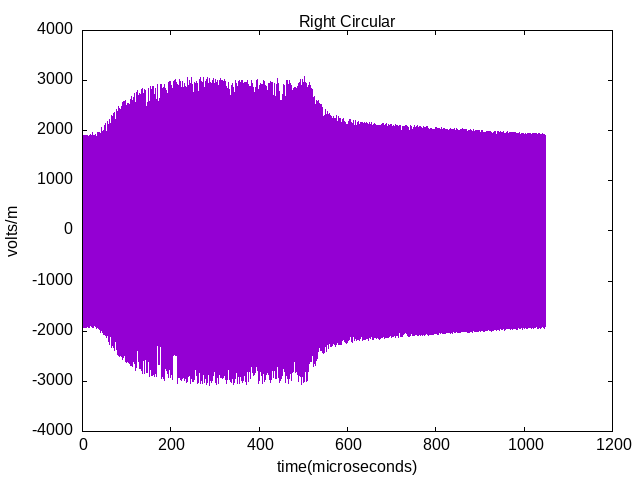
\includegraphics[width=1\textwidth]{time-aliasing.png}
                \caption{Aliasing also applies to the time domain.}
                \label{fig:time-aliasing}
            \end{figure}
        \end{column}
        \begin{column} {0.4\textwidth}
            \begin{figure}[h]
                \centering 
                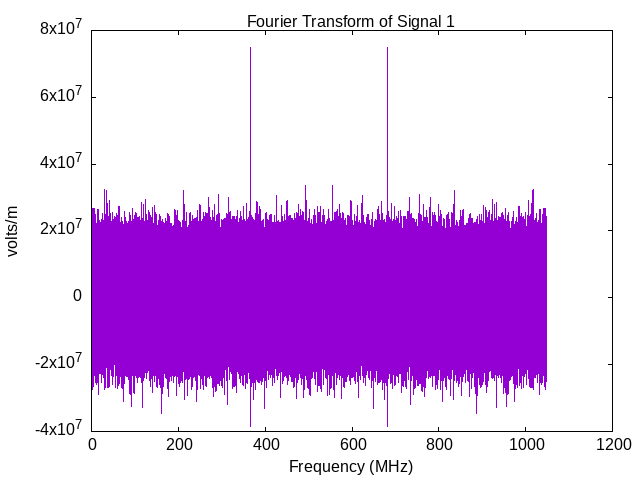
\includegraphics[width=1\textwidth]{fft_test_08.png}
                \caption{Aliasing in the frequency domain}
                \label{fig:fft-test-08}
            \end{figure}
        \end{column}
    \end{columns}
    \end{frame}
    
    \begin{frame}{Phase}
        \begin{quote}
            \huge{\textit{"Phase is the most important thing, that's why we never plot it" \\ - Ed Fenimore}}
        \end{quote}   
    \end{frame}
    
\section{Results and Discussion}

    \begin{frame}{Results}
        \begin{figure}[h]
            \centering
            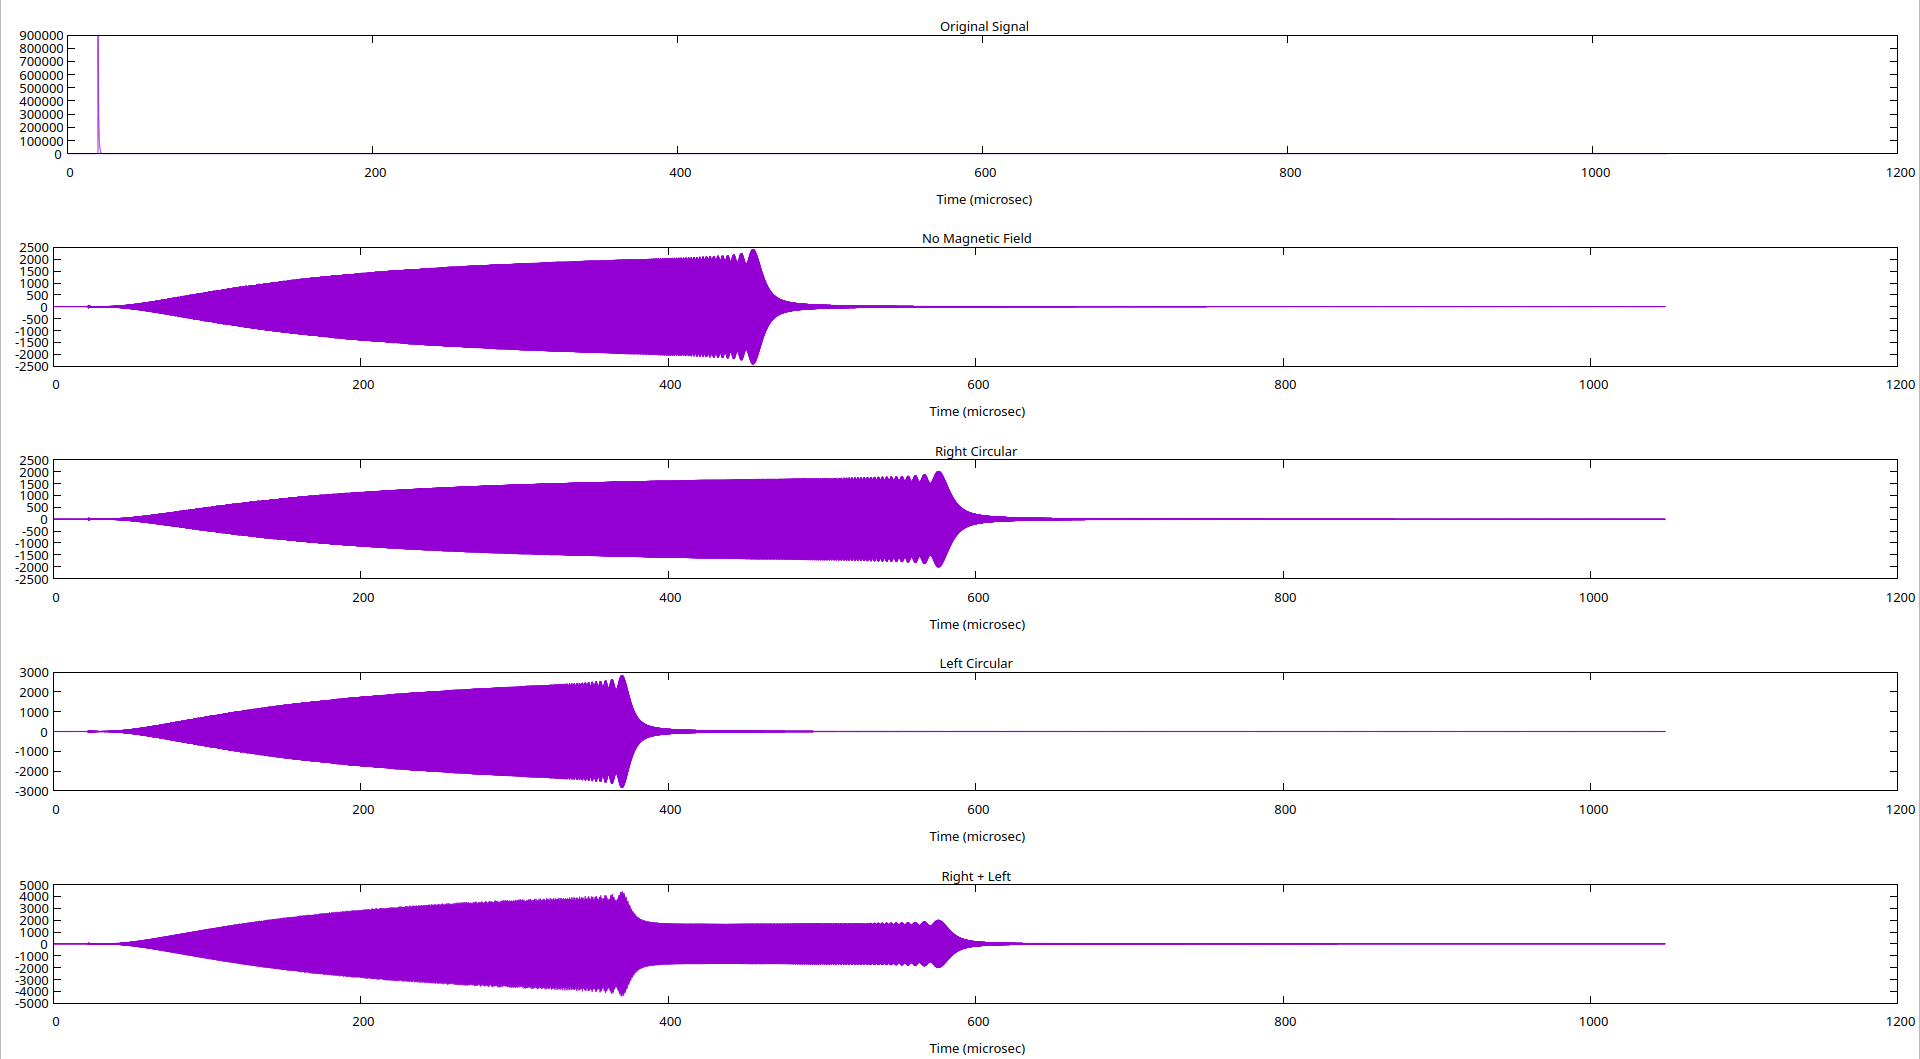
\includegraphics[width=0.6\textwidth]{signal_final_results.png}
            \caption{Final results showing right-circular, left-circular, a sum of the two, and without the magnetic field.}
            \label{fig:final-results}
        \end{figure}
    \end{frame}
    
    \begin{frame}{Modifications}
        \begin{figure}[h]
            \centering
            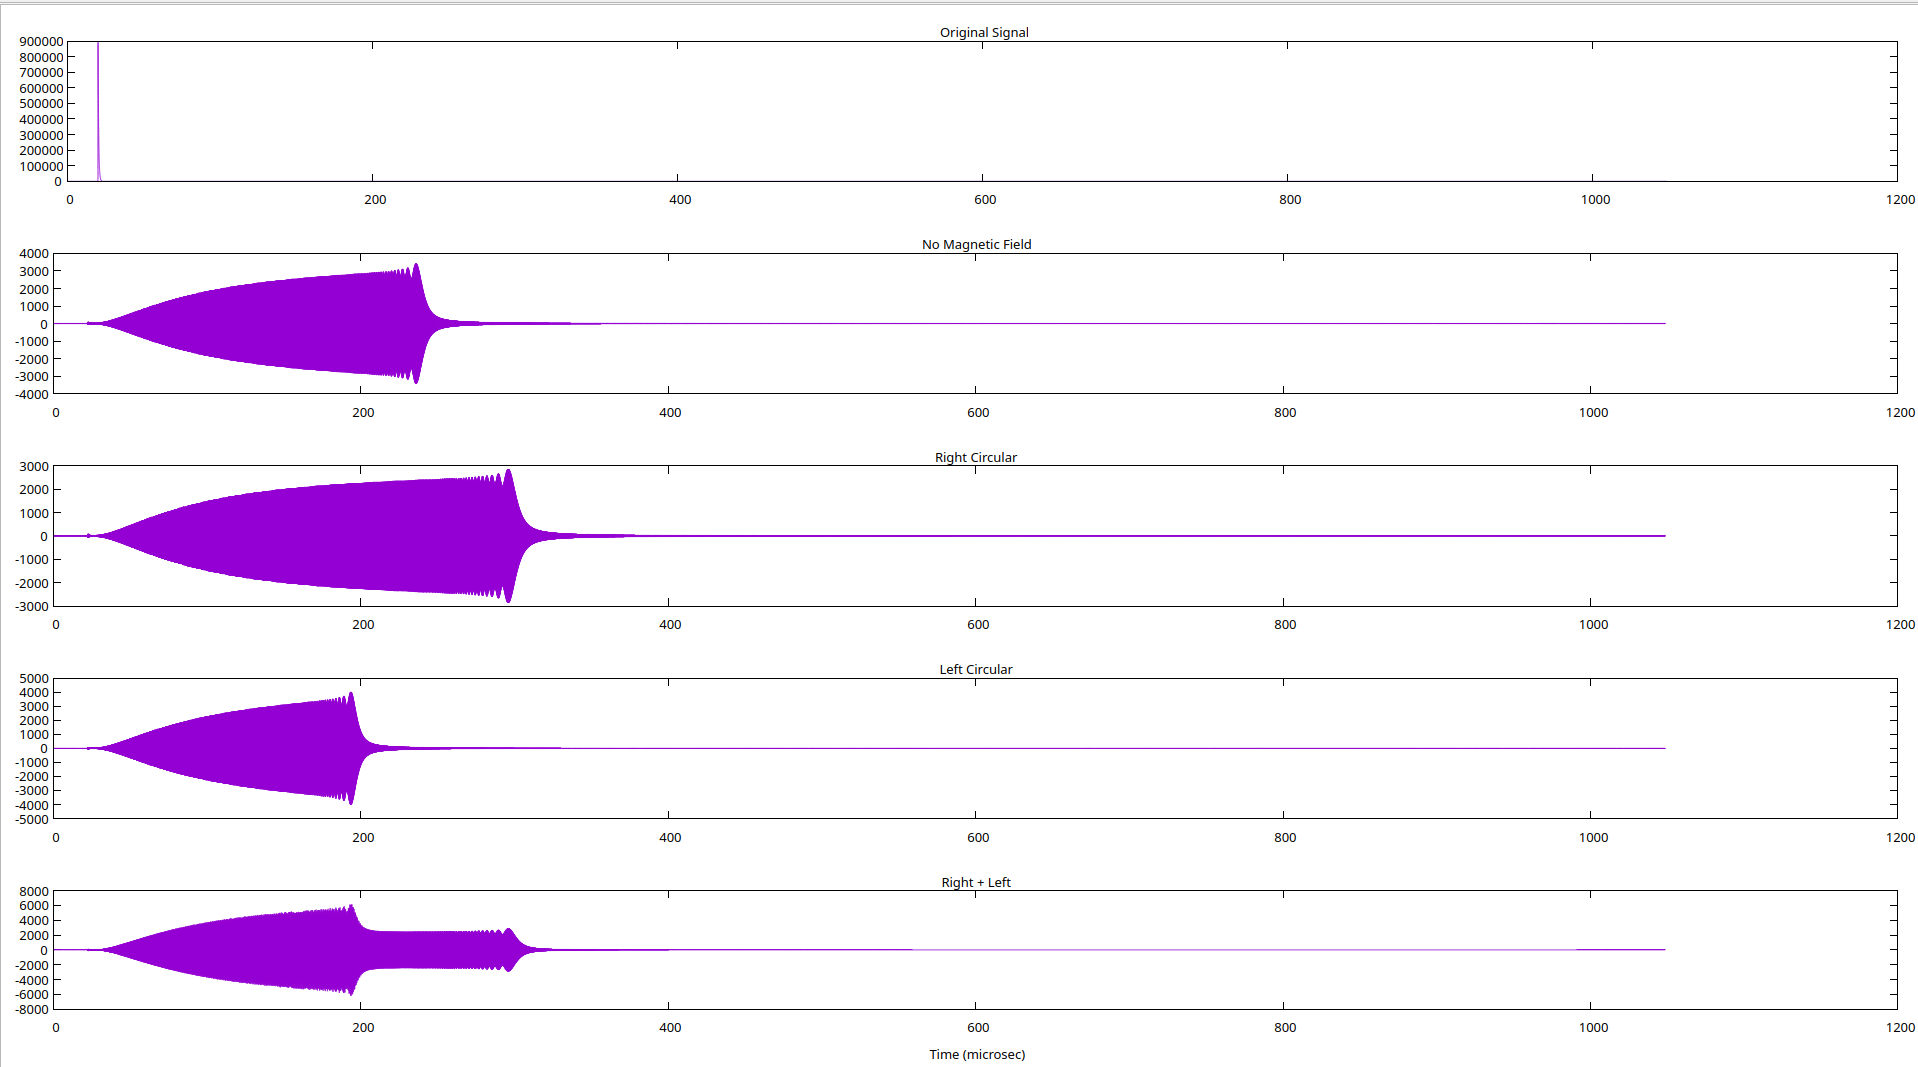
\includegraphics[width=0.6\textwidth]{signal_stec_15.png}
            \caption{Final results if the ionosphere had half the electron density.}
            \label{fig:stec-15}
        \end{figure}
    \end{frame}
    
    \begin{frame}{Limitations}
        \begin{quote}
            \Large{My main limitation was that I couldn't access real data provided by the FORTE satellite, so I approximated my own.}
        \end{quote}
    \end{frame}
    
    \begin{frame}{Further Research}
        \begin{itemize}
            \item \huge{Spectrogram
            \item Refraction
            \item Geolocation}
        \end{itemize}
    \end{frame}
   
\end{document}



//////////////////
